
% slam-formulation.tex

\documentclass[dvipdfmx,a4paper]{jsarticle}

\usepackage{docmute}

% settings.tex

\usepackage{atbegshi}
\AtBeginDvi{\special{pdf:tounicode 90ms-RKSJ-UCS2}}

\usepackage{amsmath}
\usepackage{amssymb}
\usepackage{amsfonts}
\usepackage{amsthm}
\usepackage{bm}
\usepackage{ascmac}
\usepackage{comment}
\usepackage{fancybox}
\usepackage{framed}
\usepackage{color}
\usepackage[dvipdfmx]{graphicx}
\usepackage{multicol}
\usepackage{multirow}
\usepackage{pdflscape}
\usepackage{verbatim}

\usepackage{url}
\urlstyle{same}

\DeclareMathOperator*{\argmax}{arg\,max}
\DeclareMathOperator*{\argmin}{arg\,min}
\DeclareMathOperator{\Tr}{Tr}
\DeclareMathOperator{\KL}{KL}
\DeclareMathOperator{\diag}{diag}
\DeclareMathOperator{\bel}{bel}
\DeclareMathOperator{\belp}{\overline{bel}}

\usepackage[T1]{fontenc}
\usepackage[utf8]{inputenc}

\usepackage{algorithm}
\usepackage{algpseudocode}
\usepackage{algorithmicx}

\renewcommand{\algorithmicrequire}{\textbf{Input:}}
\renewcommand{\algorithmicensure}{\textbf{Output:}}

\makeatletter
\renewcommand{\ALG@name}{アルゴリズム}
\makeatother

\algnewcommand{\Initialize}[1]{
	\State \textbf{Initialize:}
 	\State \hspace*{\algorithmicindent}\parbox[t]{0.8\linewidth}{\raggedright #1}}


\usepackage{geometry}
\geometry{left=19.05mm,right=19.05mm,top=19.05mm,bottom=19.05mm}

\title{SLAM問題の定式化}
\author{にゃーん}
\date{\today}

\begin{document}

\maketitle

\section{SLAM問題の分類}
SLAM\~(スラム)はSimultaneous Localization And Mappingの略称であり、自己位置推定と地図構築を同時に行う問題である。移動ロボットが、周囲の環境の地図を持たず、また自己の姿勢も分からないという状況にあるとき、環境の地図を構築しながら、その地図上での自己位置を推定しなければならない。しかし、ロボットが計測データを使って地図を生成するためには、ロボットの自己位置が必要であり、またロボットの自己位置を推定するためには地図が必要である。即ち、自己位置推定と地図構築は相互依存の関係にあるため、SLAMの問題を解くのは一層困難になる。

\subsection{オンラインSLAM問題}
SLAM問題は、\textbf{オンラインSLAM問題}(Online SLAM)と\textbf{完全SLAM問題}(Full SLAM)の2種類に分けられる~\cite{Thrun07}\cite{Hara16}。オンラインSLAM問題では、時刻$t$における姿勢$x_t$地図$m$の事後確率$p(x_t, m | z_{1 : t}, u_{1 : t})$を求める。オンラインSLAMはその名の通り、各時刻において事後確率を求める、逐次的なアルゴリズムである。以下の漸化式を利用すれば、時刻$t$における事後確率$p(x_t, m | z_{1 : t}, u_{1 : t})$を、時刻$t - 1$における事後確率$p(x_{t - 1}, m | z_{1 : t - 1}, u_{1 : t - 1})$から求められる。ベイズフィルタの導出と同様にして、漸化式は次のように得られる。
\begin{eqnarray}
	&& p(x_t, m | z_{1 : t}, u_{1 : t}) \nonumber \\
	&=& \frac{p(z_t | x_t, m, z_{1 : t - 1}, u_{1 : t - 1}) p(x_t, m | z_{1 : t - 1}, u_{1 : t - 1})}{p(z_t | z_{1 : t - 1}, u_{1 : t - 1})} \qquad (\because ベイズの定理) \\
	&=& \eta \ p(z_t | x_t, m, z_{1 : t - 1}, u_{1 : t - 1}) p(x_t, m | z_{1 : t - 1}, u_{1 : t - 1}) \\
	&=& \eta \ p(z_t | x_t, m) p(x_t, m | z_{1 : t - 1}, u_{1 : t})
\end{eqnarray}
ここで$\eta = p(z_t | z_{1 : t - 1}, u_{1 : t - 1})$は、現在の状態$x_t$と地図$m$には依存しないため、定数項として扱っている。最後の式変形では、現在の計測$z_t$は、現在の姿勢$x_t$と地図$m$によって決まり、それ以外の変数($z_{1 : t - 1}, u_{1 : t - 1}$)とは独立であることを利用している。右側の項$p(x_t, m | z_{1 : t - 1}, u_{1 : t})$は次のように、変数$x_{t - 1}$に関する周辺化として記述される。
\begin{eqnarray}
	&& p(x_t, m | z_{1 : t - 1}, u_{1 : t}) \nonumber \\
	&=& \int p(x_t, x_{t - 1}, m | z_{1 : t - 1}, u_{1 : t}) dx_{t - 1} \\
	&=& \int p(x_t | x_{t - 1}, m, z_{1 : t - 1}, u_{1 : t}) p(x_{t - 1}, m | z_{1 : t - 1}, u_{1 : t}) dx_{t - 1} \\
	&=& \int p(x_t | x_{t - 1}, u_t) p(x_{t - 1}, m | z_{1 : t - 1}, u_{1 : t - 1}) dx_{t - 1}
\end{eqnarray}
最後の式変形では、マルコフ性の仮定から、現在の状態$x_t$は、直前の状態$x_{t - 1}$と制御$u_t$のみに依存し、従ってそれ以外の変数($m, z_{1 : t - 1}, u_{1 : t}$)とは独立であることを利用している。また時刻$t - 1$における状態$x_{t - 1}$は、未来の時刻$t$における制御$u_t$とは関係ないことも利用している。地図$m$が現在の状態$x_t$の推定に何らかの有益な情報をもたらす場合、$x_t$は$m$とは独立にはならず、$p(x_t | x_{t - 1}, u_t) \neq p(x_t | x_{t - 1}, u_t, m)$となる。しかし、ここでは$x_t$が$m$とは独立と仮定している。このとき漸化式は以下のようになる。
\begin{equation}
	p(x_t, m | z_{1 : t}, u_{1 : t}) = \eta \ p(z_t | x_t, m) \int p(x_t | x_{t - 1}, u_t) p(x_{t - 1}, m | z_{1 : t - 1}, u_{1 : t - 1}) dx_{t - 1}
\end{equation}
漸化式には、状態遷移確率$p(x_t | x_{t - 1}, u_t)$と計測確率$p(z_t | x_t, m)$の双方が含まれている。最初に制御$u_t$を用いて、直前の事後確率$p(x_{t - 1}, m | z_{1 : t - 1}, u_{1 : t - 1})$と状態遷移確率$p(x_t | x_{t - 1}, u_t)$の積を周辺化し、現在の状態$x_t$に関する予測を確率分布$p(x_t, m | z_{1 : t - 1}, u_{1 : t})$として得る。次に計測$z_t$を用いて、確率分布$p(x_t, m | z_{1 : t - 1}, u_{1 : t})$と計測確率$p(z_t | x_t, m)$との積を求め、時刻$t$における事後確率$p(x_t, m | z_{1 : t}, u_{1 : t})$を得る。即ち事後確率の更新は、予測と修正の2ステップに分けられる。制御$u_t$を使って状態$x_t$に関する予測を立てた後、計測$z_t$を使って予測を修正し、かつ現在の地図$m$に対する推定を行う。これよりオンラインSLAM問題は、拡張カルマンフィルタやパーティクルフィルタのような、ベイズフィルタの枠組みで計算できる。\newline

オンラインSLAM問題は、図\ref{fig:online-slam}に示すような確率モデルとして表現される。図\ref{fig:online-slam}では、現在の状態$x_t$は直前の状態$x_{t - 1}$と制御$u_t$にのみ依存することと、計測$z_t$は現在の状態$x_t$と地図$m$にのみ依存することの両方が表現される。状態遷移確率$p(x_t | x_{t - 1}, u_t)$と計測確率$p(z_t | x_t)$の形から、変数間の依存関係は明らかである。またオンラインSLAM問題において推定したい変数は、図\ref{fig:online-slam}では濃い灰色で囲われている。

\subsection{完全SLAM問題}
完全SLAM問題では、時刻$t$における姿勢$x_t$ではなく、全時刻における軌跡$x_{1 : t}$に対して、事後確率が計算される。事後確率は$p(x_{1 : t}, m | z_{1 : t}, u_{1 : t})$のように表され、オンラインSLAMにおける事後確率$p(x_t, m | z_{1 : t}, u_{1 : t})$との関係は、以下のように周辺化として記述される。
\begin{equation}
	p(x_t, m | z_{1 : t}, u_{1 : t}) = \int \int \cdots \int p(x_{1 : t}, m | z_{1 : t}, u_{1 : t}) dx_1 dx_2 \cdots dx_{t - 1}
\end{equation}
完全SLAM問題は、Rao-Blackwellizedパーティクルフィルタ(FastSLAM)やGraphSLAMを用いて解くことができる。前者は完全SLAM問題をオンラインで、後者はオフラインで解くアルゴリズムである。また前者はベイズフィルタ、後者は非線形最適化ベースの手法である。完全SLAM問題は、図\ref{fig:full-slam}に示すような確率モデルとして表現される。変数間のグラフ構造は先程の図\ref{fig:online-slam}と同一のものである。完全SLAMにおいて推定したいのは、ロボットの完全な軌跡$x_{1 : t}$と地図$m$であり、それらの変数が濃い灰色で囲われている。

\subsection{SLAM問題の難しさ}
上記では地図$m$の具体的な表現法については言及されなかった。地図の1つとして、レーザースキャナ(レーザレンジファインダ)から得られるスキャンデータ(点群)を貼り合わせて作られる、点群地図(Point cloud map)が挙げられる。点群地図を用いるとき、スキャンデータ$z_t$を構成する各点が、地図上のどの点と対応するのか判定する必要がある。このようなスキャンデータと地図の対応関係を、変数$c_t$として明示的に導入するのは有効である。対応付け変数$c_t$を用いると、オンラインSLAM問題における事後確率は$p(x_t, m, c_t | z_{1 : t}, u_{1 : t})$、完全SLAM問題の事後確率は$p(x_{1 : t}, m, c_{1 : t} | z_{1 : t}, u_{1 : t})$のように表される~\cite{Thrun07}\cite{Tomono16}\cite{Tomono18}。\newline

SLAMでは、連続空間における姿勢$x_t$や地図$m$の推定(非線形最適化やフィルタ処理)だけでなく、離散的な対応付け変数$c_t$の推定、言い換えるとスキャンデータと地図の対応付け問題(組み合わせ最適化問題)を解く必要がある。このようにSLAMには連続的な問題と離散的な問題の双方が含まれている。連続的なパラメータ$x_t, m$、離散的なパラメータ$c_t$の個数は、普通どちらも大きくなる。非線形最適化により$x_t, m$を求める場合、次元数が大きくなると局所解に陥りやすくなる。また取り得る全ての対応付け$c_{1 : t}$の場合の数は、時刻$t$が大きくなるに従って指数的に増加する。これより解の候補は莫大になり、事後分布を厳密に求めることは不可能となる~\cite{Thrun07}\cite{Tomono16}\cite{Tomono18}。

\begin{figure}[htbp]
	\centering
	\includegraphics[keepaspectratio, scale=0.5]{figures/online-slam.pdf}
	\caption{オンラインSLAM問題の確率モデル}
	\label{fig:online-slam}
\end{figure}

\begin{figure}[htbp]
	\centering
	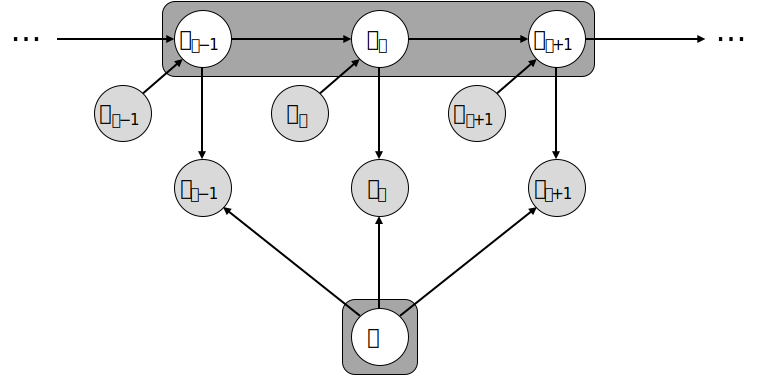
\includegraphics[keepaspectratio, scale=0.5]{figures/full-slam.pdf}
	\caption{完全SLAM問題の確率モデル}
	\label{fig:full-slam}
\end{figure}

\newpage

\bibliographystyle{plain}
\bibliography{slam-formulation}

\end{document}
